
\section{Factorization of rate equations}
See \cite{noor2013note} for details. The flux of a reaction can be factorized into three
conceptually distinct terms: kinetic ($F_K$), thermodynamic ($F_T$) and regulatory ($F_R$),
as shown in Equation \ref{eq:flux_factorization}.
\begin{equation}
    v = F_K \times F_T \times F_R
    \label{eq:flux_factorization}
\end{equation}

Assuming that saturation and regulation effects can be ignored, i.e. the enzyme is substrate
saturated, and if $\Delta_r G' \leq 0$, the forward flux can be expressed as in Equation \ref{eq:thermokinetic_flux_forward}.
\begin{equation}
    v_\text{forward} \leq \underbrace{\text{kcat} \times E_i}_{F_K} \times \underbrace{\left(1 - \exp \left( \frac{\Delta_r G'}{RT} \right)\right)}_{F_T}
    \label{eq:thermokinetic_flux_forward}
\end{equation}

Likewise, if $\Delta_r G' \geq 0$, the backward flux can be expressed as Equation \ref{eq:thermokinetic_flux_backward}.
\begin{equation}
    v_\text{backward} \leq -\underbrace{\text{kcat}' \times E_i}_{F_K} \times \underbrace{\left(\exp \left( \frac{-\Delta_r G'}{RT}\right) - 1\right)}_{F_T}
    \label{eq:thermokinetic_flux_backward}
\end{equation}

Taken together, the flux of a reaction can be bounded by Equation \ref{eq:thermokinetic_flux_bound},
with the $\min$ and $\max$ ensuring that the thermodynamic factors are well behaved.
\begin{equation}
    \text{kcat}' \times E_i \times \min{\left(0, \exp \left( \frac{-\Delta_r G'}{RT}\right) - 1\right)} \leq v \leq \text{kcat} \times E_i \times \max \left(0, 1 - \exp \left( \frac{\Delta_r G'}{RT} \right)\right)
    \label{eq:thermokinetic_flux_bound}
\end{equation}

Assuming that the forward and reverse $\text{kcat}$'s are the same, and that flux is always
at its boundary (parsimonious enzyme usage), Equation \ref{eq:thermokinetic_flux_bound} can be
simplified to Equation \ref{eq:thermokinetic_flux_simplified}.
\begin{equation}
    v = \text{kcat} \times E_i \times \text{sign}\left(\Delta_r G' \right) \times \left(1 - \exp \left( \frac{-|\Delta_r G'|}{RT} \right)\right)
    \label{eq:thermokinetic_flux_simplified}
\end{equation}

Furthermore, to avoid the usage of indicator variables in the subsequent optimization
problems, the thermodynamic term will be approximated, as shown in Equation
\ref{eq:thermokinetic_tanh_approximation}, where $p$ is a fitting variable.
\begin{equation}
    \tanh \left(p \cdot x \right) \approx  \text{sign}\left( x \right) \times \left(1 - \exp \left( x \right)\right)
    \label{eq:thermokinetic_tanh_approximation}
\end{equation}

The fit is shown in Figure \ref{fig:tanh_approximation}.
\begin{figure}[H]
    \centering
    \includegraphics[width=\textwidth]{imgs/tanh_approximation.pdf}
    \caption{Fit of Equation \ref{eq:thermokinetic_tanh_approximation} where $p=-0.7$.}
    \label{fig:tanh_approximation}
\end{figure}

\section{Thermokinetic algorithm}
It is desirable to combine the MOMENT algorithm \cite{adadi2012prediction} with thermodynamic
constraints, since such a formulation will necessarily be more physiologically representative
of the underlying cellular metabolism. Equation \ref{eq:thermo_moment} shows this formulation,
including the thermodynamic approximation of Equation \ref{eq:thermokinetic_tanh_approximation}.
\begin{equation}
\begin{aligned}
& \underset{E, c, \Delta_r G^0}{\text{maximize}}
& & c^T v \\
& \text{subject to}
& & S v = 0 \\
& & & \Delta_r G_i = \Delta_r G_i^0 + R T \sum_j\nu_j\log\left(c_j \right) \\
& & & v_i = \text{kcat}_i \times E_i \times \tanh \left(\frac{\Delta_r G_i}{RT} \right)\\
& & & \sum_i E_i \leq \text{protein fraction}\\
& & & c_{j, \text{LB}} \leq c_j \leq c_{j, \text{UB}}\\
\end{aligned}
\label{eq:thermo_moment}
\end{equation}
Where $c$, $v$, and $S$ retain their usual meaning from FBA, $E_i$ is the enzyme
concentration of reaction $i$. When a constraint is indexed by $i$, it applies to each
reaction in the model. Each reaction $i$ is also associated with a change in standard Gibbs free
energy, $\Delta_r G_i^0$.



\section{Thermodynamics constrains physical processes}
The first law of thermodynamics is the law of energy conservation, energy can neither be created or destroyed but that energy can only be converted from one type to another.

\begin{equation}
    \Delta Energy_surr + \Delta Energy_sys = 0  
    \label{eq:Thermo_Sys_Surr}
\end{equation}

Due to the system being closed system only work and heat can be transferred between it and the surroundings.

\begin{equation}
    \Delta Energy_surr = - Q_surr - W_surr = - Q - W
    \label{eq:Thermo_Work_Heat_1}
\end{equation}
\begin{equation}
    \Delta Energy_sys = Q_sys + W_sys = Q + W
    \label{eq:Thermo_Work_Heat_2}
\end{equation}

Conventionally energy that flows into the system is taken as positive.
In a closed system there can also be processes that lead to changes in internal energy. These changes are the sum of the changes in heat and work occurring in the system.

\begin{equation}
    U_t \equiv Q + W
    \label{eq:Thermo_U}
\end{equation}

Where $U_t$ is the total change in internal energy. The differential form of equation \ref{eq:Thermo_U} is shown in \ref{eq:Thermo_U_extended}.

\begin{equation}
    dU_t = dQ + dW 
    \label{eq:Thermo_U_small}
\end{equation}

Extensive variables $U_t$ and the volume (V) depend on the metabolites concentrations in the system. Intensive variables like temperature (T) and pressure (p) are concentration independent. Extensive and intensive variables are related through the mass (m) or the moles (n), as shown in \ref{eq:Thermo_nU} and \ref{eq:Thermo_nV}.

\begin{equation}
    U_t = mU or U_t = nU
    \label{eq:Thermo_nU}
\end{equation}
\begin{equation}
    V_t = mV or V_t = nV  
    \label{eq:Thermo_nV}
\end{equation}

With this equation \ref{eq:Thermo_U_small} can be extended to \ref{eq:Thermo_U_extended}:

\begin{equation}
    d(nU_t) = dQ + dW
    \label{eq:Thermo_U_extended}
\end{equation}

Where Q and W always pertain to the total change of heat and work.

Equation \ref{eq:Thermo_U_extended} can be used to introduce ehnthalpy H. For a closed system under going a mechanically reversible process the mole of the system can be added by equation \ref{eq:Thermo_rev}.

\begin{equation}
    dW = - Pd(nV)
    \label{eq:Thermo_rev}
\end{equation}

Assuming constant pressure eq. \ref{eq:Thermo_rev} can then substitute into eq. \ref{eq:Thermo_U_extended} to yield eq. \ref{eq:Thermo_substituted}.

\begin{equation}
    d(nU_t) = dQ - Pd(nV)
    \label{eq:Thermo_substituted}
\end{equation}

This equation can be solved for dQ as in \ref{eq:Thermo_Q_solved_1} and \ref{eq:Thermo_Q_solved_2}.

\begin{equation}
    dQ = d(nU) + Pd(nV)
    \label{eq:Thermo_Q_solved_1}
\end{equation}
\begin{equation}
    dQ = d(n(U + PV))
    \label{eq:Thermo_Q_solved_2}
\end{equation}

Defining enthalpy as H $\equiv$ U + PV, the heat transferred to a system can be described by eq. \ref{eq:Thermo_Enthalpy} under the condition of constant pressure.

\begin{equation}
    \fbox{dQ = d(nH)}
    \label{eq:Thermo_Enthalpy}
\end{equation}

The second law of thermodynamics deals with entropy. In general the total change in entropy due to a process, as shown in \ref{eq:Thermo_Entropy} can never be negative.

\begin{equation}
    \fbox \Delta S_total \geq 0}
    \label{eq:Thermo_Entropy}
\end{equation}

A consequence of \ref{eq:Thermo_Entropy} is that every process will only happen in the direction where the total entropy change is not negative. This is also limited by a value of 0 for reversible reactions. 

\section{Gibbs free energy}
Gibbs free energy change of a reaction can be derived by combining the first and second law of thermodynamics. Here the reaction is assumed to be in thermal and mechanical equilibrium with it's surroundings. Hence, both temperature (T) and pressure (p) are constant.

The entropy change of the surroundings is shown in eq. \ref{eq:Gibbs_Entropy}.

\begin{equation}
    dS_surr = - dQ/T
    \label{eq:Gibbs_Entropy}
\end{equation}

The 2nd law dictates that the total change of entropy - the sum for the surroundings and the system - has to be non-negative:

\begin{equation}
    dS_t + dS_surr \geq 0 
    \label{eq:Gibbs_Enthalpy}
\end{equation}

Substituting \ref{eq:Gibbs_Entropy} into \ref{eq:Gibbs_Enthalpy} and simplifying yields \ref{eq:Gibbs_Q}.

\begin{equation}
    dS_t - dQ/T \geq 0
    \label{eq:Gibbs_0}
\end{equation}
\begin{equation}
    dQ \leq TdS_t
    \label{eq:Gibbs_Q}
\end{equation}

The first law can be used to substitute dQ as ahown in \ref{eq:Gibbs_U} and \ref{eq:Gibbs_dQ}:

\begin{equation}
    U_t = dQ + dW = dQ - Pd(nV_t)
    \label{eq:Gibbs_U}
\end{equation}
\begin{equation}
    dQ = dU_t + PdV_t
    \label{eq:Gibbs_dQ}
\end{equation}

Combining the equations \ref{eq:Gibbs_Q}, \ref{eq:Gibbs_dQ} and rearranging of the equation:

\begin{equation}
    dU_t + PdV_t \leq TdS_t
    \label{eq:Gibbs_dU_t}
\end{equation}
\begin{equation}
    dU_t + PdV_t - TdS_t \leq 0
    \label{eq:Gibbs_leq_0}
\end{equation}

Substituting U + PV with H.

\begin{equation}
    dH - TdS_t \leq 0 (4.9)
    \label{eq:Gibbs_dH}
\end{equation}

Assuming constant T, \ref{eq:Gibbs_dH} can be written as \ref{eq:Gibbs_dG} . It can be substituted with G.

\begin{equation}
    \fbox{G = H - TS}
    \label{eq:Gibbs_G}
\end{equation}
\begin{equation}
    dG $\leq$ 0 
    \label{eq:Gibbs_dG}
\end{equation}

Equation \ref{eq:Gibbs_dG} shows that any spontaneous reaction will lead to a decrease of Gibbs free energy if they happen under constant pressure and temperature. Thus $\Delta$G can be used to predict the direction of a reaction.

\section{Self replicator model}
This self replicator model is a coarse grained representation of cellular metabolism. It consists of passive transporters, ribosomes, metabolic enzymes and enzymes for lipid synthesis enzymes. 

The model employs Mechaelis-Menten-kinetics for the reaction rates and is based on several physiological assumptions. The cell has a limited intracellular density, which constrains the amount of ribosomes, metabolic enzymes and lipid synthesis enzymes that can be present in the cell. The growth rate of the cell is limited by the membrane proportions, which consists of the surface to area ratio $\beta$ and the composition of the membrane namely the ratio of transporters and lipids, where the amount of transporters can not be higher than that of the lipids. This is so the structural integrity of the cell can be simulated because a real cell would generally not be able to survive with a membrane that consists of more transporters and other enzymes than lipids. 

\begin{figure}[H]
    \centering
    \includegraphics[width=\textwidth]{imgs/Molenaar.pdf}
    \caption{Scheme of the basic seflreplicator model consisting of the most important parts.}
    \label{fig:Molenaar}
\end{figure}

In this model the precursor is used as the educt for both the lipid and enzyme synthesis. The lipid synthesising enzyme uses the precursor to create the lipids for the cell membrane while the ribosomes use it to create all the enzymes including the ribosomes them self. Due to the ribosomes producing not only the transporters, lipid synthesising enzymes, the enzymes used for metabolic reactions but also themselves this model is considered a self replicator model. 

This basic model does not take overflow metabolism into account, it introduces the basic structure and boundaries for the model, to show the underlining relationships between the different parts. The model shows that there is a direct correlation between the substrate concentration and the growth rate. Specifically that an increase in substrate abundance leads to a higher growth rate, which occurs because at low substrate concentrations the cell has need of a lot more transporters to increase the chance of them coming into contact with a substrate molecule. 

The connection between a growth rate and substrate concentration shown by this model in figure 2.1 can also be seen in the experimental data from \cite{schulze1964} in figure 2.2. This shows that the model behaves in a way that resembles in vivo data.

\begin{figure}[H]
    \centering
    \includegraphics[width=\textwidth]{imgs/fig2com.PNG}
    \caption{1. The results of the model, showing that with an increase of the substrate concentration the growth rate increases up to a certain point where it starts to plateau. 2. Experimental data from \cite{schulze1964} which shows a similar behaviour to the data from the model, meaning this is not just a random behaviour in the model.}
    \label{fig:fig2com}
\end{figure}

\ref{fig:Figure_3Cband} With a higher substrate concentration the chance of a transporter interacting with a substrate molecule rises, thus the cell can now spend more resources for other processes leading to a higher growth rate.
In the model these processes would be more synthesis of metabolic enzymes, ribosomes, lipid synthesis enzymes, as well as lipids. This shift in enzyme concentrations inside the cell can also be seen in the model.

\begin{figure}[H]
    \centering
    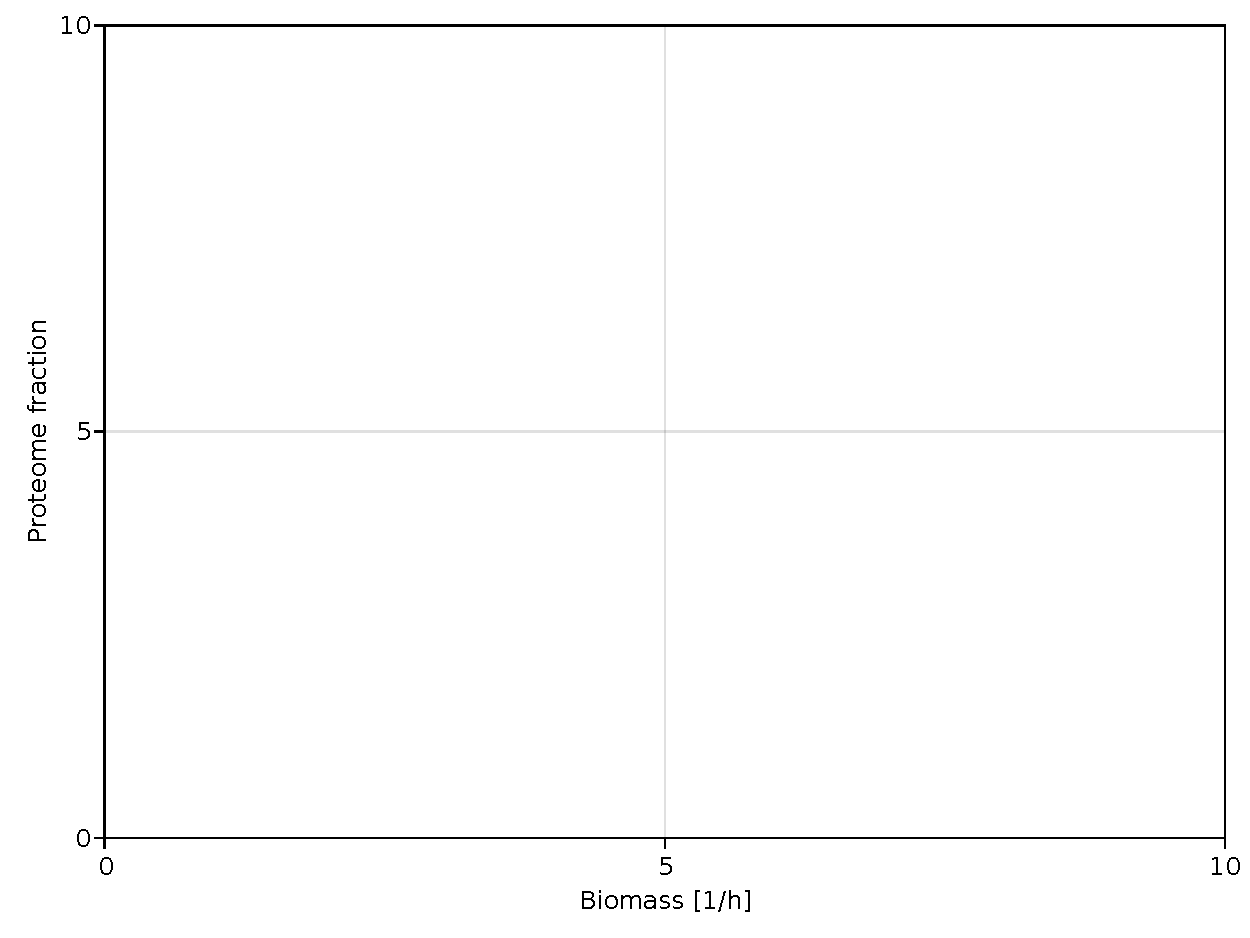
\includegraphics[width=\textwidth]{imgs/Figure_3Cband.pdf}
    \caption{}
    \label{fig:Figure_3Cband}
\end{figure}

The lipid synthesis enzymes plateau fast due to the cell only being able to grow at a specific maximum rate, anything above that would be risking the integrity of the cells stability. The amount of metabolic enzyme increases as well so that the increasing concentration of substrate inside the cell can be used effectively. But the increase in the production for these enzymes forces the cell to drastically increase the amount of ribosomes, so that the total enzyme amounts can be upheld over a long period of time. 
This increase in overall enzyme synthesis by the ribosomes - and thus the growth rate - also means that a higher rate in ribosome activity is observable.

\begin{figure}[H]
    \centering
    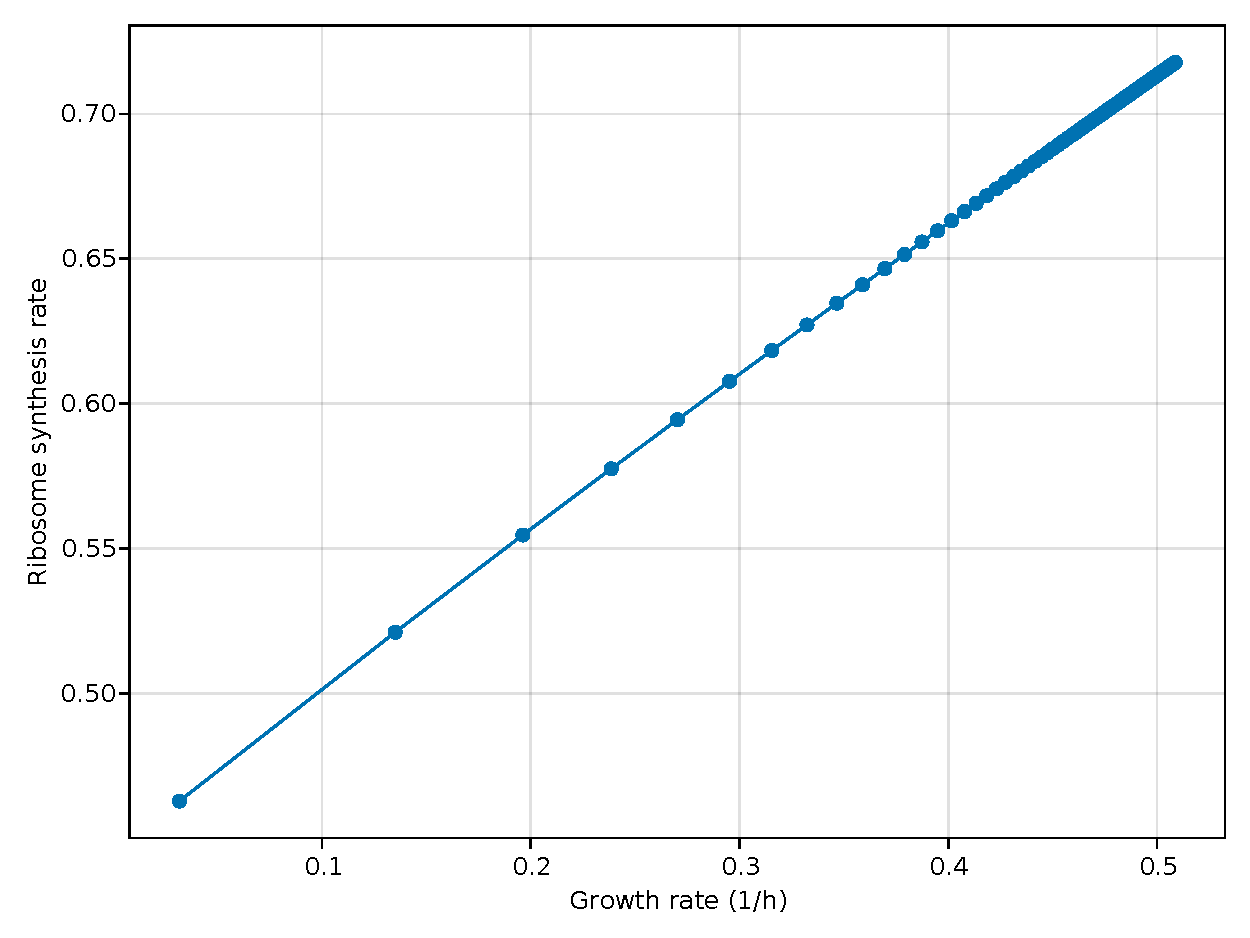
\includegraphics[width=\textwidth]{imgs/Figure_3E.pdf}
    \caption{An increase in growth rate is linked to an increase in ribosome synthesis rate.}
    \label{fig:Figure_3E}
\end{figure}

\section{Transporters}
Transporters are a group of membrane proteins that facilitate the diffusion/transport of molecules across the lipid membrane of cells. These proteins can be broadly categorized into three groups, passive, primary active and secondary active. The difference between these is what process they utilize to power the substrate transport. Passively substrate can only flow from a high concentration to a lower one, while active transport can work against these gradients with the use of energy

Small, lipophilic molecules can cross the lipid membrane by simple diffusion along the concentration gradient. For bigger and hydrophilic molecules this is not possible, thus cell have two types of passive transporter to allow those molecules to diffuse. 

\begin{figure}[H]
    \centering
    \includegraphics[width=\textwidth]{imgs/Passive.pdf}
    \caption{A scheme of the three types of passive transport. from right to left: carrier protein, channel protein, simple diffusion. Also shown is the concentration gradient for a substrate.}
    \label{fig:Passive}
\end{figure}

One of those are channel proteins which are pores in the membrane. These pores have a hydrophilic inside, providing a substrate nonspecific way inside the cell for hydrophilic molecules. Another protein for passive transport are Carrier proteins. These are substrate specific and work by having that substrate bind to it. This leads to a change in the proteins confirmation pushing the substrate through and opening up on the other side.

The active transport is a way to work around the concentration gradients for molecules. Primary active transporters do that by using the energy released by hydrolysis of ATP to ADP and phosphate. For this the ATP binds to a transporter and when the substrate also binds this leads to a conformation change. Through hat change both the hydrolysis and the transport of the substrate to the other side are forced. The energy released is needed to enact the confirmation change. 
This kind of transport generally happens either as a uniport where one substrate is transported or as a contraport. A contraport transports two different substrates against their respective gradients in opposite directions.

\begin{figure}[H]
    \centering
    \includegraphics[width=\textwidth]{imgs/PActive.pdf}
    \caption{Scheme of primary active transport. Both uniport and contraport as well as the corresponding concentration gradients are shown.}
    \label{fig:PActive}
\end{figure}

Secondary active transport is another way to transport a substrate against its concentration gradient. The difference between primary and secondary active transport is that the secondary active transport does not use energy in for of ATP. It uses the coupling of the transport two substrates. one is transported with its gradient the other one against it. For this both of the substrates need to bind to the protein which then leads to a change in conformation. 

\begin{figure}[H]
    \centering
    \includegraphics[width=\textwidth]{imgs/SActive.pdf}
    \caption{Scheme of secondary active transporters. Shown are antiport and symport.}
    \label{fig:SActive}
\end{figure}

Secondary active transport can happen as an antiport where the two substrates are transported to opposite side of the membrane. It can also happen as a symport, where both of them are transported to the same side. 